\documentclass[conference]{IEEEtran}

\usepackage[T1]{fontenc}

\usepackage[utf8]{inputenc}

\usepackage{amsmath,amssymb}

\usepackage{graphicx}

\usepackage{booktabs}

\usepackage{url}

\usepackage{cite}

\usepackage{array}

\usepackage{microtype}

\usepackage{capt-of}

\graphicspath{{latex_figures/}}

\title{Comparative Evaluation of PWL Retinex and Established Low-Light Enhancement Methods}

\author{\IEEEauthorblockN{Toney Williams}}

\begin{document}

\maketitle

\begin{abstract}Low-light image enhancement improves visibility, but methods trade image fidelity against training and inference requirements. This paper compares the published piecewise-linear (PWL) Retinex method with Retinex-DIP, LiCENt, EnlightenGAN, KinD, and LIME. Paired image quality is evaluated on LOL-v1 and LOL-v2 Real using PSNR, SSIM, RGB MAE, VIF, and CIEDE2000. No-reference quality is assessed on DICM, the LIME image collection, NPE, and VV with NIQE, BRISQUE, NIQMC, and BLIINDS-II. A separate ExDark experiment applies one fixed detector and reports image-label accuracy, macro precision, and confusion matrices for all six methods on the same balanced subset. PWL improves on Retinex-DIP across paired means and performs favorably against LIME on several measures, while learned methods lead on most paired metrics. In the detector experiment, Retinex-DIP has the highest image-label accuracy and PWL the highest macro precision. These results support PWL as a training-independent method with metric-specific strengths, not as a universal image-quality leader.\end{abstract}

\begin{IEEEkeywords}low-light image enhancement, Retinex, piecewise-linear approximation, image-quality assessment, downstream detection.\end{IEEEkeywords}

\section{INTRODUCTION}

Low-light image enhancement (LLIE) seeks to reveal details obscured by insufficient illumination while maintaining color, edges, and structure. This balance matters in applications such as surveillance and autonomous systems, where degraded input can affect both human interpretation and downstream vision. Embedded use adds constraints on computation, memory, and predictability.

Retinex methods represent an image through illumination and reflectance, then adjust illumination while retaining scene detail. Upadhyay and Sarawadekar's PWL Retinex approximates the exponential edge weights in its illumination filter with an eight-segment piecewise-linear function [1]. Its fixed operations avoid offline network training. This makes it a useful baseline for asking whether a deterministic Retinex method can remain competitive with newer learning-based approaches.

We compare PWL Retinex with Retinex-DIP, LiCENt, EnlightenGAN, KinD, and LIME, a set drawn from the supplied comparative study and the methods' primary papers [2]--[7]. Paired-reference quality is evaluated on LOL-v1 and LOL-v2 Real; blind quality predictors are evaluated on four unpaired image collections. ExDark is used separately to study downstream detector response. We report metric-specific results and limit conclusions to measurements retained for this comparison.

\section{RELATED WORK}

Classical low-light enhancement includes histogram adjustment and illumination-map methods. LIME estimates an initial illumination map from the maximum color-channel intensity and refines it with a structure-aware prior [7]. Unlike learned enhancement networks, it uses a hand-designed optimization procedure and provides a training-free comparison point.

Learning-based methods represent several distinct design choices. Retinex-DIP uses an image-specific deep prior and optimizes its representation for each test image [3]. KinD uses a learned Retinex decomposition with separate reflectance-restoration and illumination-adjustment stages [6]. LiCENt processes the HSL light channel with a learned enhancement model [4], while EnlightenGAN uses unpaired adversarial learning with global and local discriminators [5]. These differences affect both how the methods are trained and how they are used at inference.

The PWL method is the model-based Retinex baseline in this comparison [1]. Its fixed piecewise-linear approximation targets a predictable illumination-filter computation. The comparison paper that informed method selection summarizes related Retinex and deep-learning approaches [2], while this study evaluates the selected methods under a shared LOL-v1 scoring pipeline rather than combining scores copied from different publications.

The methods were selected to span model-based illumination estimation, classical optimization, image-specific deep priors, and learned enhancement networks. PWL Retinex and LIME operate without offline model training, Retinex-DIP optimizes a deep prior per test image, and LiCENt, EnlightenGAN, and KinD use learned model parameters. These categories differ in training and inference requirements, so the analysis discusses them alongside image-quality scores without treating training cost as an image-quality metric.

Full-reference scores and no-reference scores answer different questions. The paired LOL datasets measure agreement with aligned normal-light targets, whereas blind metrics estimate image quality from an output alone. Such predictors can reward natural-image statistics without ensuring faithful exposure or color reconstruction. Reporting both kinds of evidence helps expose trade-offs, but their numerical scales should not be combined into a single overall score.

\section{METHODOLOGY}

\subsection{Datasets}

LOL-v1 provides low-light images paired with corresponding normal-light references [8]. This benchmark supports direct evaluation of pixel fidelity, structural similarity, visual-information retention, and perceptual color difference. LOL-v2 Real provides an additional paired benchmark with real captured illumination variations. Both are used for full-reference comparison so method rankings can be checked across distinct paired collections.

The unpaired evaluation uses DICM, the LIME image collection, NPE, and VV. These collections contain low-light scenes without aligned normal-light targets, so they support blind quality estimation rather than pixelwise fidelity tests. The LIME collection is a dataset and should not be confused with the LIME enhancement algorithm. NPE was designed for non-uniform illumination [12], while the four collections provide varied real-scene content used in low-light enhancement benchmarking [11]. ExDark provides image-category labels and object annotations for dark scenes [9]; without paired bright references, it is reserved for the downstream detector experiment.

Using paired and unpaired data broadens evaluation while preserving the distinction between their roles. LOL-v1 and LOL-v2 Real permit direct comparison with aligned normal-light targets. DICM, the LIME collection, NPE, and VV extend observation to scenes without such targets, where only blind predictors are available. ExDark is included for a separate task-level probe because its labels allow detector decisions to be summarized. The ExDark experiment does not replace image-quality evaluation, and its detector scores are not treated as reference-based enhancement accuracy.

\subsection{Compared Methods}

PWL Retinex models an input image as the product of reflectance and illumination, $I(x)=R(x)L(x)$. The method estimates illumination using a local edge-preserving filter. Its weight is $w(x,y)=\beta(x,y)\exp(-|G(x)-T(y)|^2/(2\sigma^2))$, where $\beta$ gates contributions according to the method’s local minimum condition. The exponential weight is approximated by eight linear segments [1]. After estimating illumination, reflectance is recovered by division and the illumination is adjusted before recombination. This fixed pipeline requires no offline training.

\begin{equation}I=R\odot L\tag{1}\end{equation}

\begin{equation}I_{\mathrm{enh},c}(x)=R_c(x)L_{\mathrm{mod}}(x),\quad R_c(x)=\frac{I_c(x)}{L(x)}\tag{2}\end{equation}

LIME estimates illumination as $T_0(x)=\max_c I_c(x)$, then refines $T_0$ with a spatial-structure penalty and corrects the input by the refined illumination [7]. Retinex-DIP represents the image as $R\odot L$ and optimizes a deep prior separately for each input, rather than applying only an offline-trained checkpoint [3].

\begin{equation}T_0(x)=\max_c I_c(x),\quad \hat I_c(x)=\min\left(1,\frac{I_c(x)}{\hat T(x)^\gamma}\right)\tag{3}\end{equation}

KinD decomposes the image into reflectance and illumination, then applies learned reflectance restoration and illumination adjustment [6]. LiCENt uses the HSL light channel as the input to its released enhancement network [4]. EnlightenGAN generates enhanced images using an unpaired adversarial objective with global and local discrimination [5]. The supplied checkpoints were evaluated as provided; these models were not retrained for this study.

The methods differ in where their correction is applied. LIME explicitly estimates a spatial illumination map, while Retinex-family approaches separate illumination from reflectance. KinD makes this decomposition part of a learned pipeline and includes reflectance restoration. LiCENt focuses enhancement on lightness information in HSL space. EnlightenGAN learns a mapping from low-light examples without aligned paired targets, using global and local adversarial supervision. Retinex-DIP obtains an image-specific solution by optimizing a network prior for the input. These descriptions explain the comparison categories; they do not imply identical runtime or resource requirements.

\begin{equation}\text{Retinex-DIP: }\theta^*=\arg\min_\theta\mathcal{L}(G_\theta(z),I),\quad \text{LiCENt/KinD: }\hat I=f_\theta(I)\tag{4}\end{equation}

\subsection{Experimental Setup}

The same method implementations and scoring code are used on LOL-v1 and LOL-v2 Real. Per-image paired scores are summarized by their means. Five-pass results are averaged per image before the dataset mean is calculated; LiCENt is represented by one deterministic pass of its released checkpoint, and this difference is stated alongside the results. Standard-deviation values are omitted from the comparison tables as requested. The PWL scores are obtained from the software method implementation, not bit-accurate RTL output.

For unpaired analysis, NIQE and BRISQUE are calculated from method outputs, and NIQMC and BLIINDS-II are evaluated with the metric implementations used in the retained results. Dataset-level means are first computed and then averaged equally across DICM, LIME, NPE, and VV. Available outputs vary across method/dataset combinations; consequently, these unpaired macro-averages are descriptive and are not a fully matched per-image statistical comparison.

Paired image scores are computed image by image and then averaged within each dataset. The reported five-pass results use the mean of available passes for each image before aggregation; LiCENt contributes a single deterministic inference pass from its released checkpoint. For blind metrics, each dataset contributes one mean to the equally weighted macro-average, so a collection does not dominate simply because it contains more images. Since output coverage differs across methods, these summaries describe available evidence and are not a controlled paired significance test.

For ExDark, a fixed pretrained Torchvision SSDLite320 MobileNetV3 detector is applied with the same weights and input processing to each method output [10]. The detector's top-confidence mapped category is compared with the ExDark image label; a missing mapped detection is counted as incorrect. All six methods are scored on the same balanced subset from the official test split. Retinex-DIP uses 20 per-image optimization steps in this CPU run; its paired-image evaluation used a longer optimization, so these downstream results are interpreted separately.

\subsection{Performance Metrics}

PSNR is derived from mean squared error (MSE) between reference R and enhanced image I; larger PSNR indicates lower pixel error. SSIM compares local luminance, contrast, and structure. RGB MAE is calculated on the 8-bit channel scale, with lower values indicating smaller average absolute error.

\begin{equation}\mathrm{MSE}=\frac{1}{N}\sum_i(R_i-I_i)^2,\quad \mathrm{PSNR}=10\log_{10}\left(\frac{\mathrm{MAX}^2}{\mathrm{MSE}}\right)\tag{5}\end{equation}

\begin{equation}\mathrm{SSIM}(x,y)=\frac{(2\mu_x\mu_y+C_1)(2\sigma_{xy}+C_2)}{(\mu_x^2+\mu_y^2+C_1)(\sigma_x^2+\sigma_y^2+C_2)}\tag{6}\end{equation}

\begin{equation}\mathrm{MAE}=\frac{1}{N}\sum_i|R_i-I_i|\tag{7}\end{equation}

VIF estimates the visual information retained relative to the reference; higher values are preferred. CIEDE2000 measures perceptual color difference in CIELAB; lower values indicate closer color agreement. For ExDark, image-label accuracy is the fraction of images assigned the correct mapped category. Macro precision averages class-wise precision equally across categories. These are downstream detector measures, not generic enhancement-accuracy scores.

\begin{equation}\mathrm{Accuracy}=\frac{\sum_c\mathrm{CM}_{cc}}{N},\quad \mathrm{MacroPrecision}=\frac{1}{C}\sum_c\frac{TP_c}{TP_c+FP_c}\tag{8}\end{equation}

NIQE compares output statistics with a natural-image model and BRISQUE scores locally normalized spatial statistics; lower values are conventionally preferred. NIQMC reflects no-reference naturalness and contrast characteristics, with higher values preferred in the implementation used here. BLIINDS-II predicts distortion-related quality from transform-domain statistics, with lower scores preferred. These blind metrics are estimates, not measurements of accuracy against a bright reference.

\section{RESULTS AND DISCUSSION}

\subsection{LOL-v1 Paired Image Quality}

Tables I and II summarize the six methods on the paired benchmarks using five full-reference measures. The reported numbers are per-image means. The LOL-v1 figure shows observed minimum-to-maximum per-image ranges, not standard deviations or run-to-run variation.

\begin{table*}[!t]
\centering
\caption{MEAN FULL-REFERENCE SCORES ON LOL-V1}
\small
\setlength{\tabcolsep}{5pt}
\begin{tabular}{lrrrrr}
\toprule
Method & PSNR $\uparrow$ & SSIM $\uparrow$ & MAE $\downarrow$ & VIF $\uparrow$ & $\Delta E_{00}$ $\downarrow$ \\
\midrule
PWL Retinex & 13.73 & 0.510 & 54.57 & 0.463 & 21.41 \\
Retinex-DIP & 11.62 & 0.483 & 67.75 & 0.461 & 25.96 \\
LiCENt & 18.11 & 0.527 & 30.53 & 0.479 & 14.77 \\
EnlightenGAN & 17.54 & 0.653 & 34.21 & 0.494 & 14.43 \\
KinD & 17.69 & 0.772 & 31.23 & 0.465 & 12.44 \\
LIME & 13.11 & 0.359 & 50.09 & 0.485 & 22.27 \\
\bottomrule
\end{tabular}
\end{table*}

\begin{table*}[!t]
\centering
\caption{MEAN FULL-REFERENCE SCORES ON LOL-V2 REAL}
\small
\setlength{\tabcolsep}{5pt}
\begin{tabular}{lrrrrr}
\toprule
Method & PSNR $\uparrow$ & SSIM $\uparrow$ & MAE $\downarrow$ & VIF $\uparrow$ & $\Delta E_{00}$ $\downarrow$ \\
\midrule
PWL Retinex & 17.69 & 0.503 & 32.37 & 0.473 & 14.68 \\
Retinex-DIP & 12.71 & 0.445 & 59.62 & 0.460 & 21.09 \\
LiCENt & 18.40 & 0.502 & 26.43 & 0.506 & 15.02 \\
EnlightenGAN & 18.67 & 0.678 & 27.40 & 0.547 & 13.73 \\
KinD & 20.63 & 0.819 & 22.35 & 0.531 & 9.37 \\
LIME & 11.06 & 0.322 & 61.60 & 0.534 & 27.51 \\
\bottomrule
\end{tabular}
\end{table*}

\begin{table*}[!t]
\centering
\caption{EQUAL-DATASET MEAN NO-REFERENCE SCORES}
\small
\setlength{\tabcolsep}{5pt}
\begin{tabular}{lrrrr}
\toprule
Method & NIQE $\downarrow$ & BRISQUE $\downarrow$ & NIQMC $\uparrow$ & BLIINDS-II $\downarrow$ \\
\midrule
PWL Retinex & 4.741 & 37.86 & 5.271 & 22.57 \\
Retinex-DIP & 3.464 & 15.10 & 5.169 & 13.93 \\
LiCENt & 3.293 & 12.01 & 5.301 & 11.67 \\
EnlightenGAN & 3.255 & 11.27 & 5.215 & 17.89 \\
KinD & 3.619 & 16.57 & 5.167 & 16.88 \\
LIME & 4.767 & 30.11 & 5.238 & 25.00 \\
\bottomrule
\end{tabular}
\end{table*}

For Table III, each method's dataset mean is averaged equally across DICM, LIME, NPE, and VV. Coverage differs where a method output or metric score is unavailable, so these are descriptive macro-averages rather than fully paired per-image comparisons.

\begin{figure*}[!t]

\centering

\IfFileExists{figure_1.png}{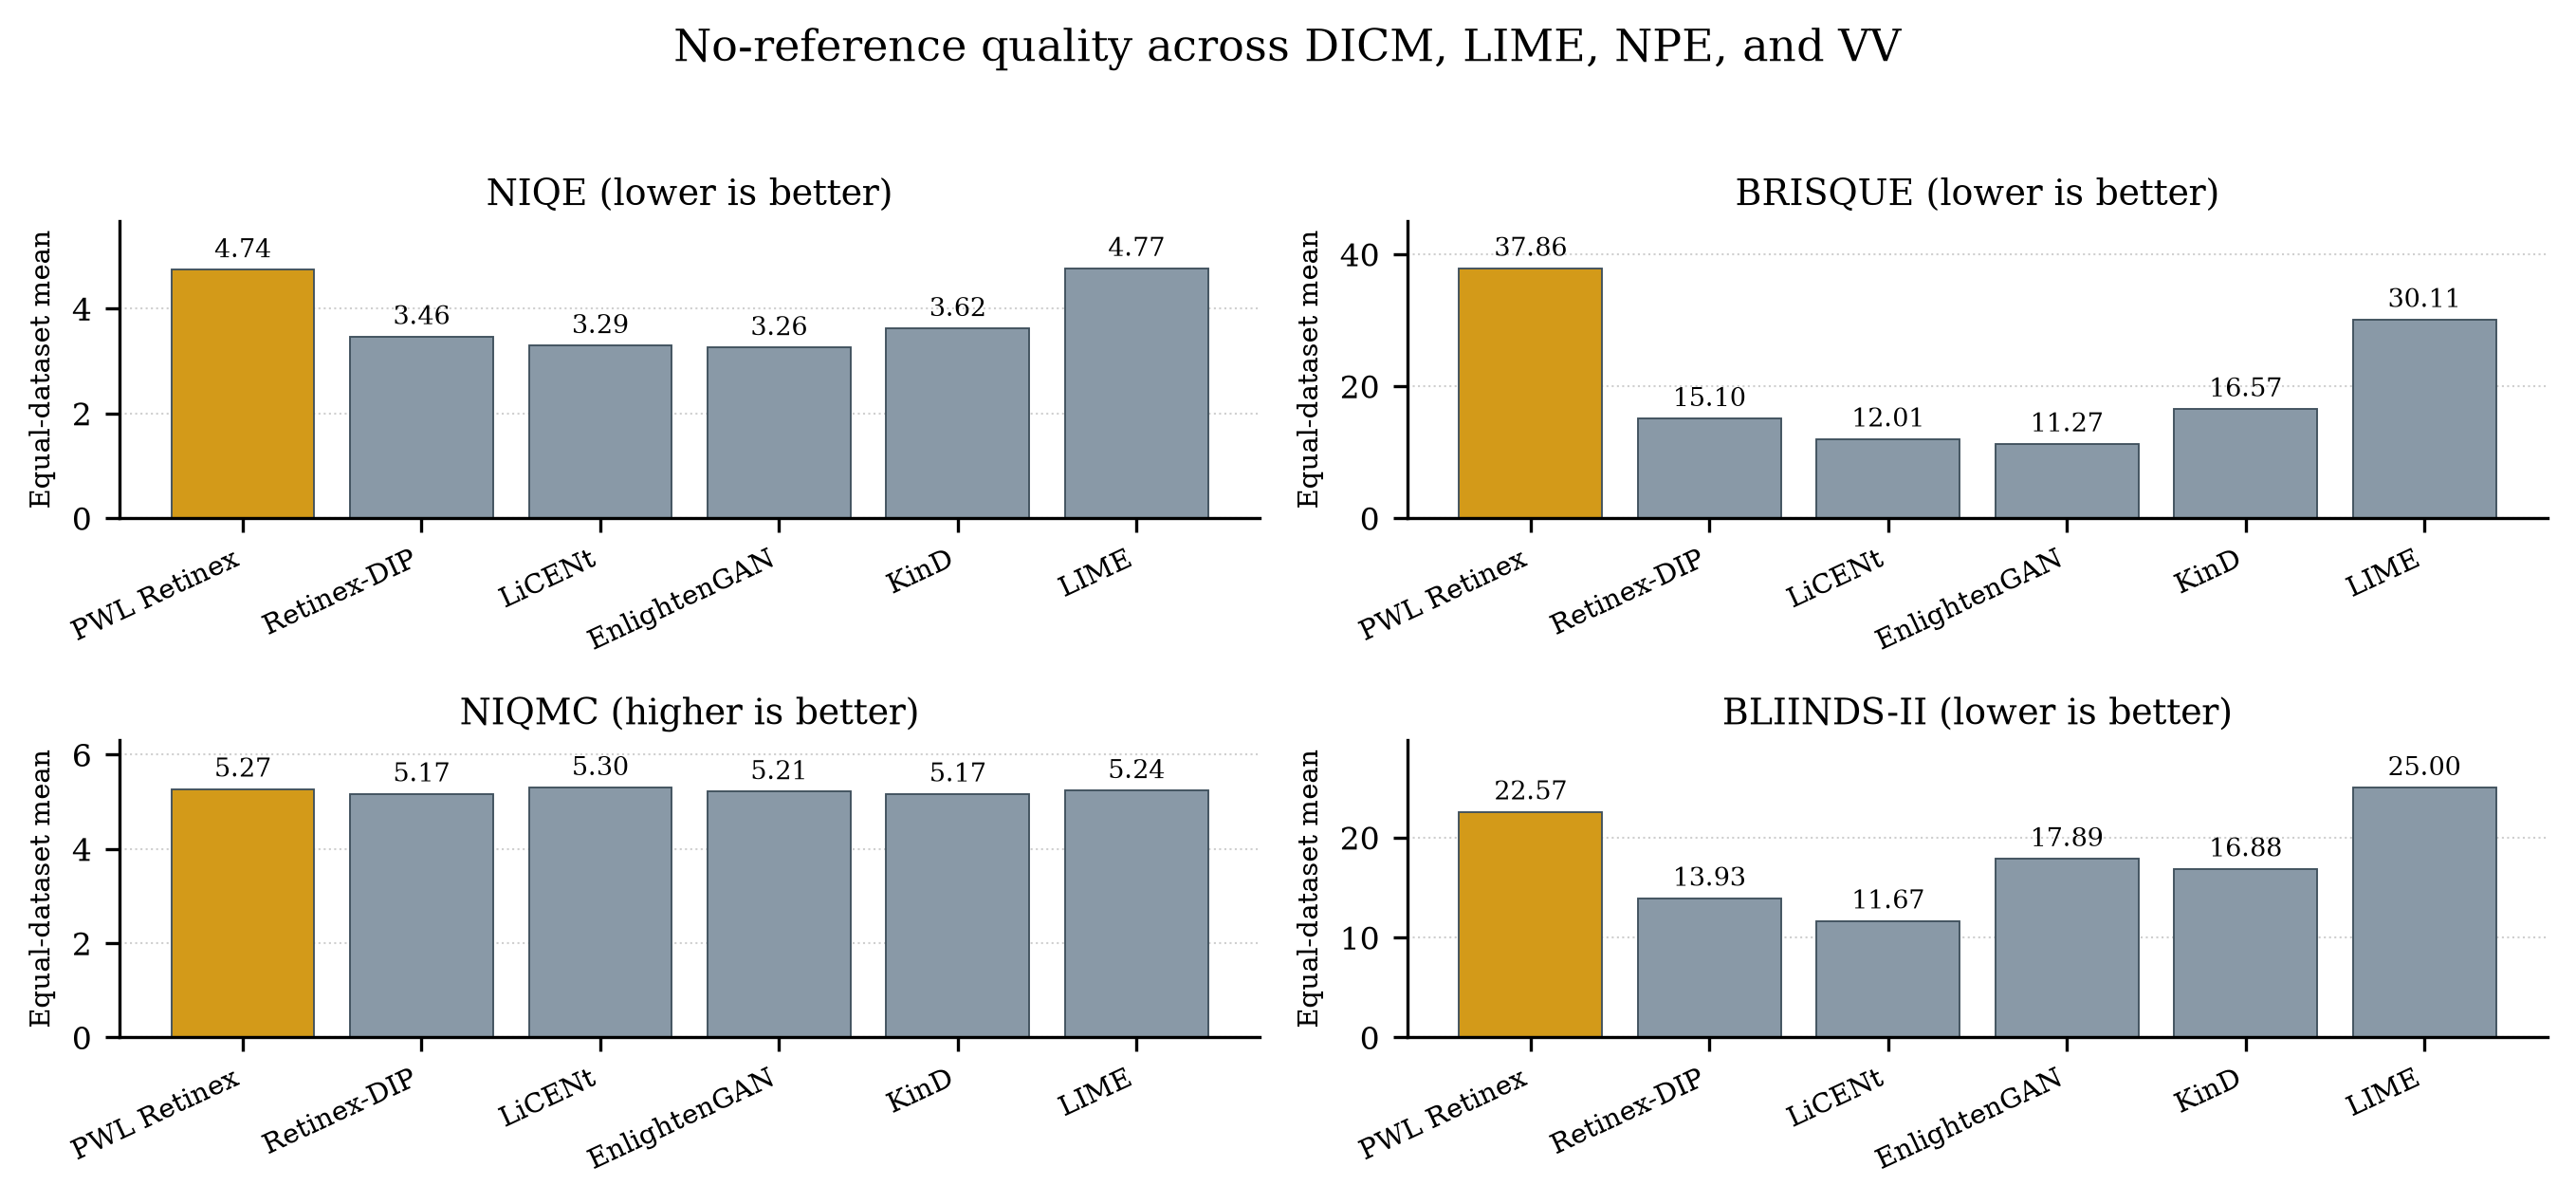
\includegraphics[width=\textwidth]{figure_1.png}}{\fbox{\parbox[c][1.1in][c]{0.9\textwidth}{\centering Figure 1 is available in the accompanying latex_figures folder.}}}

\caption{Equal-dataset mean NIQE, BRISQUE, NIQMC, and BLIINDS-II scores; no dispersion bars are shown.}

\end{figure*}

\begin{figure*}[!t]

\centering

\IfFileExists{figure_2.png}{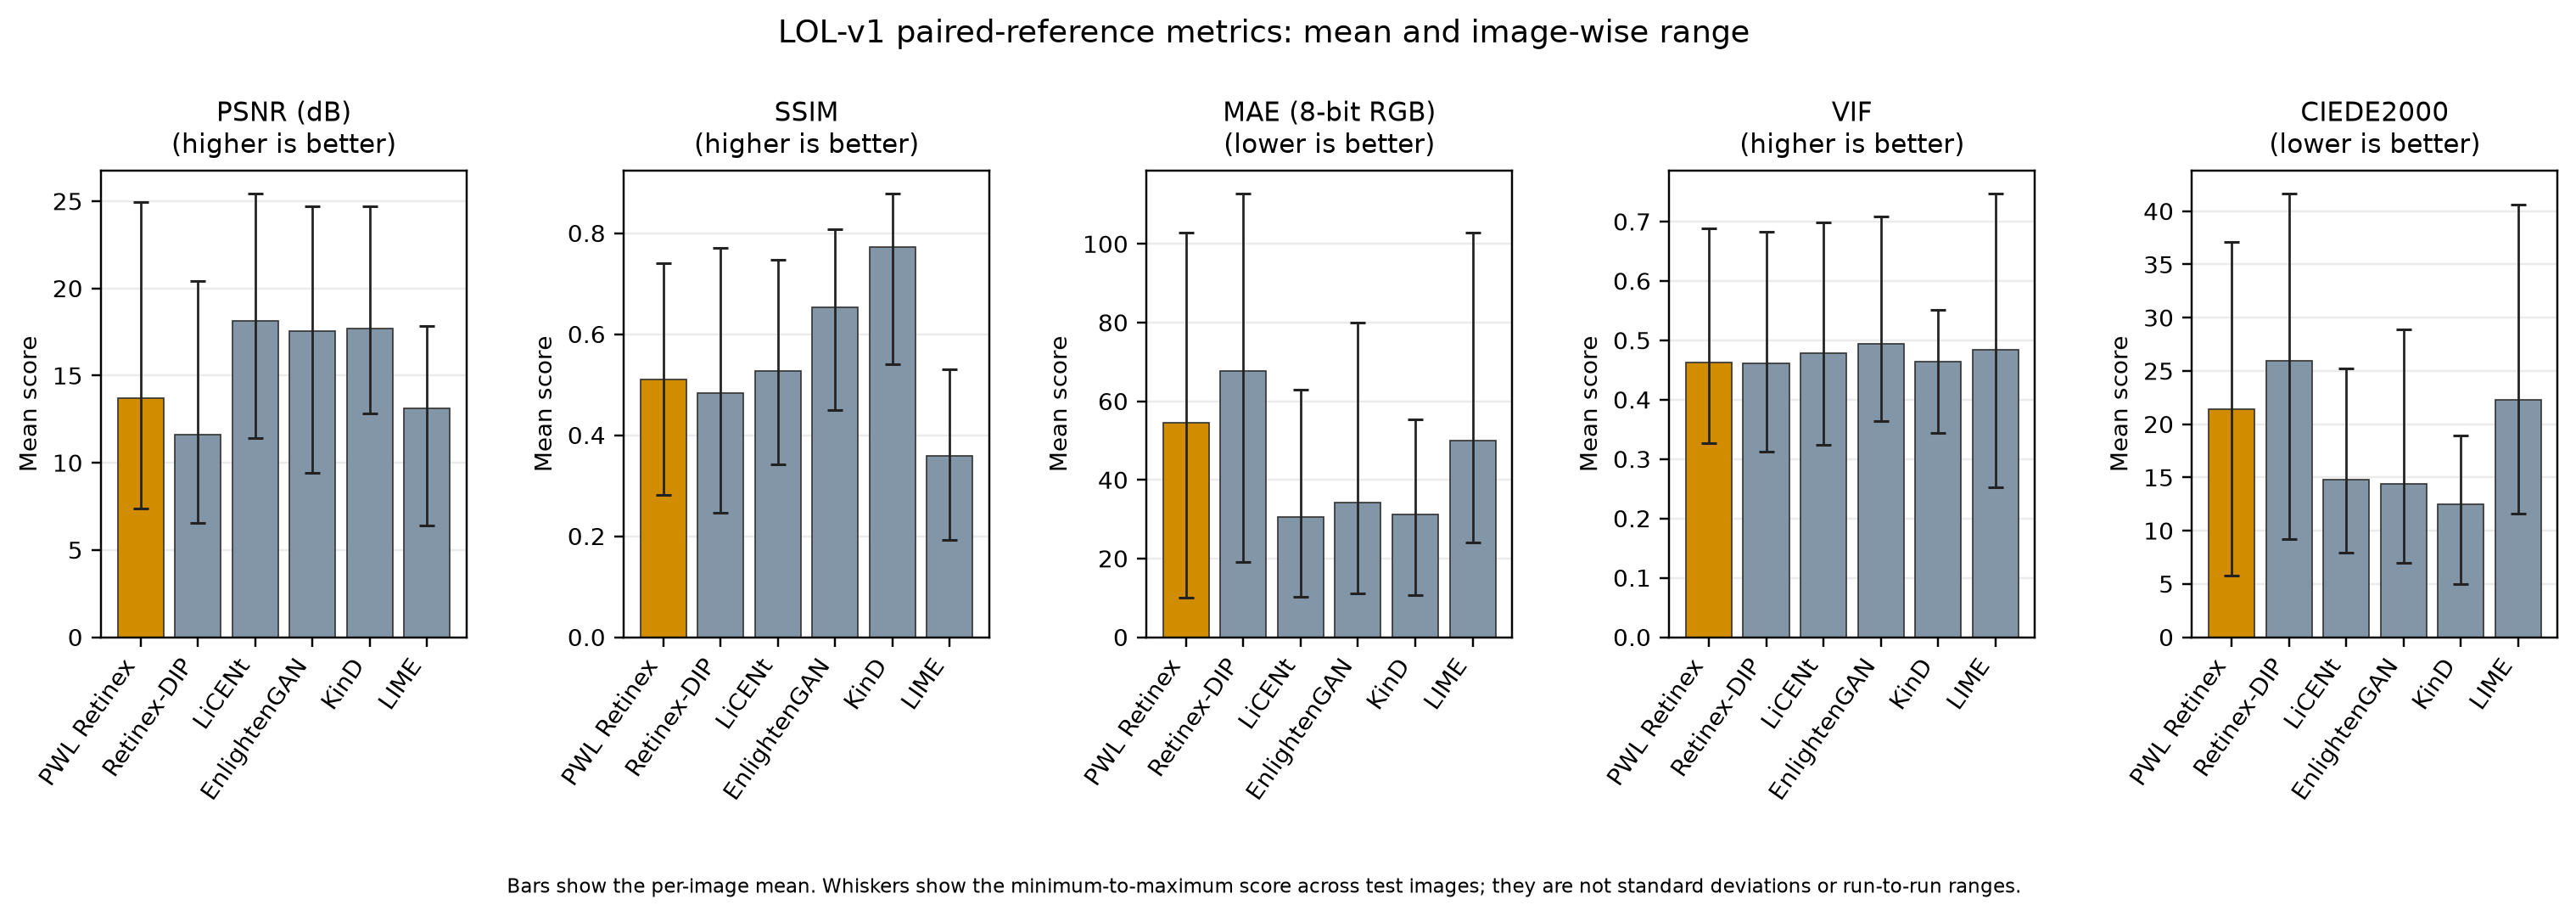
\includegraphics[width=\textwidth]{figure_2.png}}{\fbox{\parbox[c][1.1in][c]{0.9\textwidth}{\centering Figure 2 is available in the accompanying latex_figures folder.}}}

\caption{LOL-v1 metric means; whiskers show minimum-to-maximum per-image ranges.}

\end{figure*}

PWL Retinex has higher mean PSNR and SSIM, and lower MAE and CIEDE2000, than Retinex-DIP; their VIF means are nearly tied. PWL therefore compares favorably with the per-image deep-prior baseline on this test set, especially for pixel error, structure, and color difference.

Against LIME, PWL has higher PSNR and SSIM and lower CIEDE2000, while LIME has lower MAE and higher VIF. The result is mixed rather than a complete win for either method. LiCENt, EnlightenGAN, and KinD have stronger means than PWL on most or all of the listed metrics. KinD has the highest SSIM and lowest CIEDE2000; LiCENt has the highest PSNR and lowest MAE; EnlightenGAN has the highest VIF. The data do not support a universal image-quality-superiority claim for PWL.

On LOL-v2 Real, PWL again exceeds Retinex-DIP on all five means. Against LIME, it has higher PSNR and SSIM and lower MAE and CIEDE2000, while LIME has the higher VIF. Across the two paired datasets, PWL's strongest relative evidence is its consistent margin over Retinex-DIP and selected advantages over the classical illumination-map method. KinD, EnlightenGAN, and LiCENt remain stronger on several measures, including the largest structural and color-fidelity gains in the LOL-v2 table.

The LOL-v2 Real results are consistent with the main LOL-v1 pattern but also show why a single metric is insufficient. PWL raises mean PSNR over Retinex-DIP by nearly 5 dB on this benchmark and has lower pixel error and color difference, yet its SSIM remains below the stronger learned approaches. Against LIME, PWL's relative gains in PSNR, SSIM, and $\Delta E_{00}$ coexist with LIME's higher VIF. The VIF measure emphasizes retained visual information and does not necessarily rank methods in the same order as direct pixel or color error.

This comparison clarifies the practical strength of the training-independent baseline. PWL avoids offline training and has deterministic processing, while improving on Retinex-DIP and often LIME for the paired measures reported here. This may be useful where training data, model storage, or predictable deployment are constraints. These advantages remain qualitative here: uniform latency, energy, parameter-count, and memory measurements were not retained for all six methods, so no numerical quality-to-cost ranking is claimed.

These paired results should be interpreted as benchmark-specific evidence. Different capture conditions, reference alignments, and enhancement objectives can change method rankings. The reported means summarize the retained per-image scores; they do not imply that every image favors the same method. The min--max bars in Fig. 1 expose this image-to-image spread for LOL-v1 and caution against treating small differences in means as decisive without a matched statistical test.

\subsection{Unpaired No-Reference Quality}

The unpaired macro-averages show a different pattern from the paired reference metrics. PWL has the second-highest NIQMC mean, behind LiCENt, but its NIQE and BRISQUE means are higher than those of most learned methods. Its BLIINDS-II mean is also higher than the deep methods' averages, though below the LIME value. Since the metrics estimate perceptual quality from different statistical cues and the output coverage is not identical, they should be read as separate indicators rather than combined into a single score.

\subsection{ExDark Confusion Matrices and Detector Scores}

The confusion matrices in Fig. 3 compare ground-truth ExDark image categories with the top-confidence mapped category from the fixed detector. The matrices are row-normalized; the no-detection column records cases without a mapped detector output. All six methods use the same image sample and class mapping.

\begin{figure*}[!t]

\centering

\IfFileExists{figure_3.png}{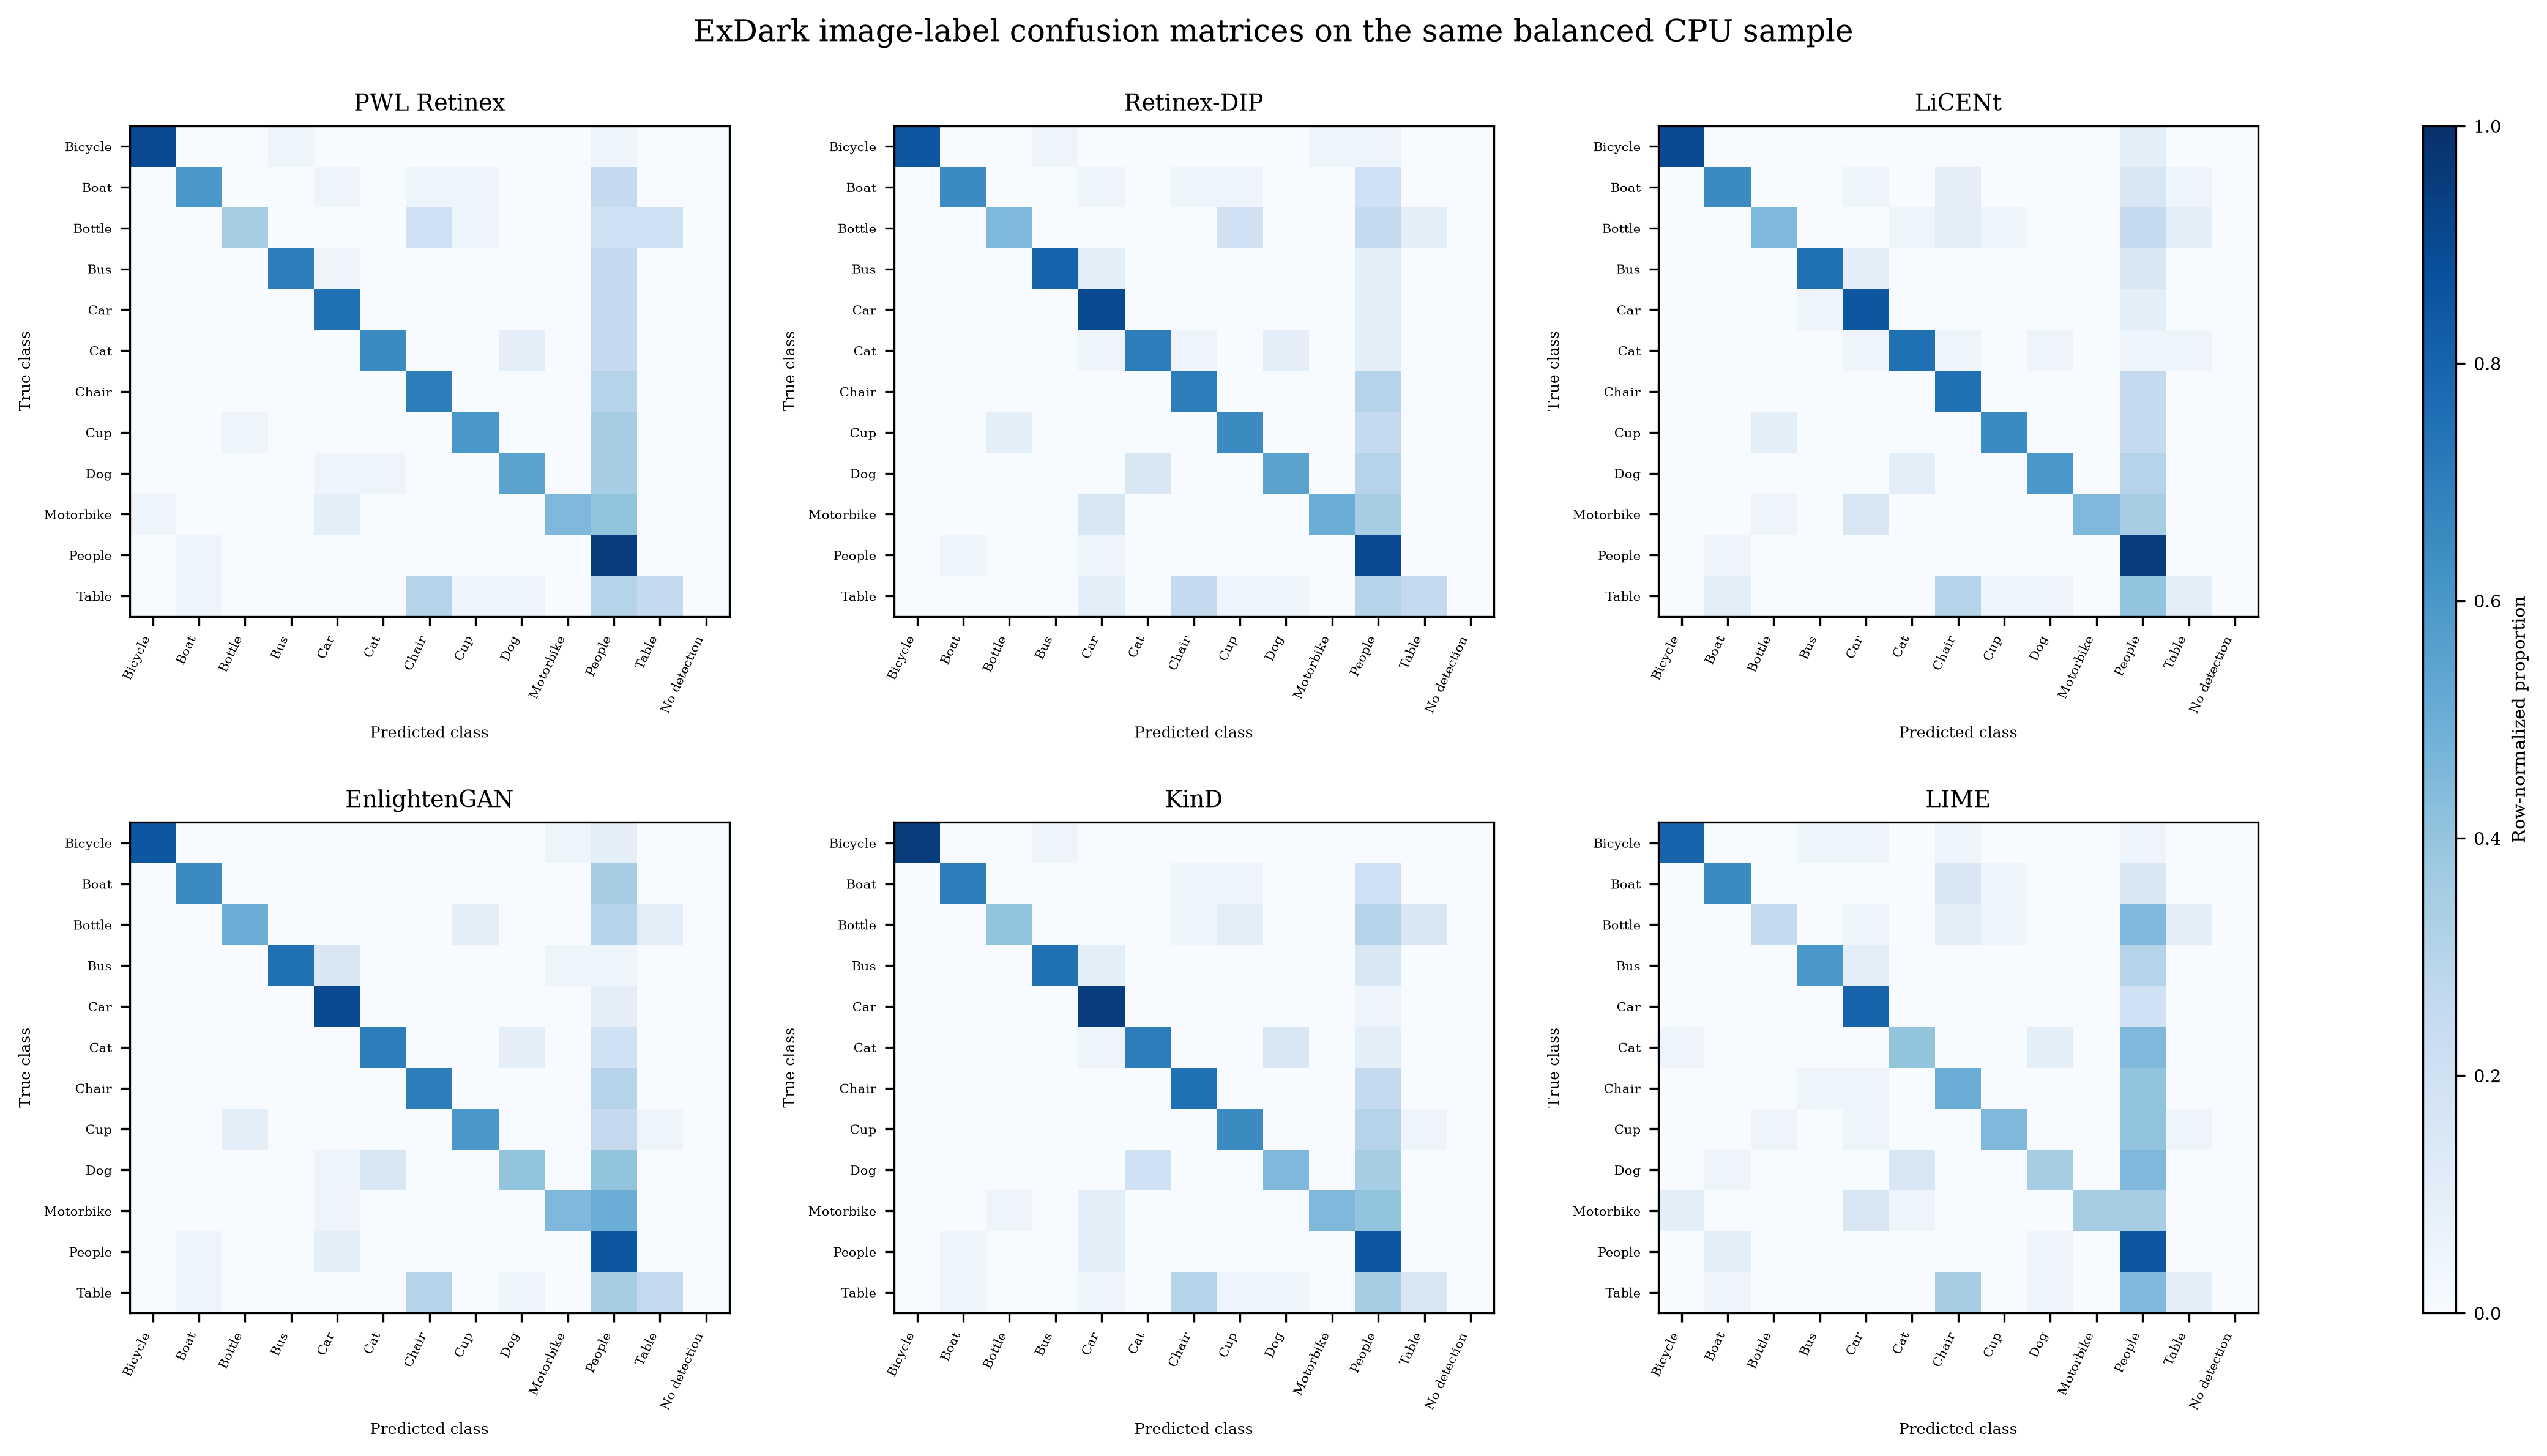
\includegraphics[width=\textwidth]{figure_3.png}}{\fbox{\parbox[c][1.1in][c]{0.9\textwidth}{\centering Figure 3 is available in the accompanying latex_figures folder.}}}

\caption{Row-normalized ExDark image-label confusion matrices for all six methods on the same balanced sample.}

\end{figure*}

\begin{table*}[!t]
\centering
\caption{EXDARK IMAGE-LABEL ACCURACY AND MACRO PRECISION}
\small
\setlength{\tabcolsep}{5pt}
\begin{tabular}{lrr}
\toprule
Method & Accuracy (\%) & Macro precision (\%) \\
\midrule
PWL Retinex & 62.08 & 76.97 \\
Retinex-DIP & 65.83 & 76.63 \\
LiCENt & 65.42 & 74.70 \\
EnlightenGAN & 63.33 & 76.65 \\
KinD & 64.58 & 74.82 \\
LIME & 50.83 & 67.35 \\
\bottomrule
\end{tabular}
\end{table*}

On this balanced sample, Retinex-DIP gives the highest image-label accuracy, followed closely by LiCENt and KinD; PWL is fourth on accuracy. PWL has the highest macro precision, narrowly above Retinex-DIP and EnlightenGAN. LIME has the lowest values among the six methods in this detector run. These outcomes reflect one frozen detector's response to enhanced images; they do not establish that enhancement improves object recognition in general.

The detector experiment is deliberately treated as a downstream response test rather than as a proxy for enhancement fidelity. A fixed detector can be sensitive to exposure, color shifts, and object prominence, but its decisions also depend on its training data and class mapping. Retinex-DIP's shortened optimization budget is a constraint specific to this CPU detector run and should be considered when interpreting its result. The confusion matrices add class-level context by showing which scene categories are most often retained or confused after enhancement.

Taken together, the evidence supports a qualified interpretation. PWL offers training-independent processing and favorable results over Retinex-DIP on both paired benchmarks, as well as selected advantages over LIME. The learning-based approaches generally achieve stronger paired-reference values, and blind metrics are mixed rather than uniformly favorable to PWL. PWL is therefore a competitive option for selected criteria, while application priorities determine whether training independence outweighs lower scores on other measures.

\subsection{Limitations and Interpretation}

Several limitations bound the conclusions. The unpaired macro-averages have unequal output coverage, Retinex-DIP uses a reduced 20-step optimization budget for the CPU detector run, and the PWL results come from the software implementation rather than bit-accurate RTL. The ExDark detector comparison uses a single balanced sample, while the paired results are reported as means and observed ranges without a significance test. Small differences should therefore be treated as descriptive unless confirmed with a matched statistical analysis.

The quality measures also encode different priorities. PSNR and MAE emphasize pixelwise error, SSIM emphasizes structure, VIF estimates retained visual information, and CIEDE2000 emphasizes perceptual color difference. Blind metrics evaluate output statistics without a bright target, while ExDark accuracy reflects one detector's behavior. No single measure captures all aspects of perceived or task-specific quality, so the results are presented metric by metric. A broader deployment decision would require matched runtime, memory, energy, and hardware measurements in addition to these image-quality results.

\section{CONCLUSION}

This paper compared PWL Retinex with five established low-light enhancement methods using paired image-quality metrics on LOL-v1 and LOL-v2 Real, no-reference metrics on DICM, LIME, NPE, and VV, and a separate detector-response evaluation on ExDark. PWL consistently exceeded Retinex-DIP on paired means and performed favorably against LIME on several paired measures. The no-reference scores were mixed: PWL ranked second in NIQMC but did not lead NIQE, BRISQUE, or BLIINDS-II. In the balanced ExDark sample, Retinex-DIP had the highest accuracy and PWL the highest macro precision; its detector result used a reduced optimization budget.

The results support PWL Retinex as a training-independent option with metric-specific strengths, particularly when avoiding offline model training is valuable. They do not show that it is the overall image-quality leader. The ExDark matrices now cover all six methods on the same sample, but further work should repeat the detector evaluation across additional balanced samples and use the full Retinex-DIP iteration budget. Further work should also validate the software PWL output against bit-accurate RTL and report computational cost under a common measurement setup.

\begin{thebibliography}{12}

\bibitem{ref1} B. B. Upadhyay and K. Sarawadekar, ``A Low Cost FPGA Implementation of Retinex Based Low-Light Image Enhancement Algorithm,'' IEEE Transactions on Circuits and Systems II: Express Briefs, vol. 71, no. 7, pp. 3503--3507, 2024, doi: 10.1109/TCSII.2024.3361561.

\bibitem{ref2} L. Kumari, N. Mittal, and M. Modi, ``Development of Optimized Adaptive Multiscale Retinex Deep Learning Model for Image Enhancement,'' IEEE Access, vol. 14, pp. 53799--53817, 2026, doi: 10.1109/ACCESS.2026.3681020.

\bibitem{ref3} Z. Zhao, B. Xiong, L. Wang, Q. Ou, L. Yu, and F. Kuang, ``RetinexDIP: A Unified Deep Framework for Low-Light Image Enhancement,'' IEEE Transactions on Circuits and Systems for Video Technology, vol. 32, no. 3, pp. 1076--1088, 2022, doi: 10.1109/TCSVT.2021.3073371.

\bibitem{ref4} A. Garg, X.-W. Pan, and L.-R. Dung, ``LiCENt: Low-Light Image Enhancement Using the Light Channel of HSL,'' IEEE Access, vol. 10, pp. 33547--33560, 2022.

\bibitem{ref5} Y. Jiang, X. Gong, D. Liu, Y. Cheng, C. Fang, X. Shen, and J. Yang, ``EnlightenGAN: Deep Light Enhancement Without Paired Supervision,'' IEEE Transactions on Image Processing, vol. 30, pp. 2340--2349, 2021.

\bibitem{ref6} Y. Zhang, J. Zhang, and X. Guo, ``Kindling the Darkness: A Practical Low-Light Image Enhancer,'' in Proceedings of the 27th ACM International Conference on Multimedia, pp. 1632--1640, 2019, doi: 10.1145/3343031.3350926.

\bibitem{ref7} X. Guo, Y. Li, and H. Ling, ``LIME: Low-Light Image Enhancement via Illumination Map Estimation,'' IEEE Transactions on Image Processing, vol. 26, no. 2, pp. 982--993, 2017, doi: 10.1109/TIP.2016.2639450.

\bibitem{ref8} C. Wei, W. Wang, W. Yang, and J. Liu, ``Deep Retinex Decomposition for Low-Light Enhancement,'' in Proceedings of the British Machine Vision Conference, 2018.

\bibitem{ref9} Y. P. Loh and C. S. Chan, ``Getting to Know Low-light Images with the Exclusively Dark Dataset,'' Computer Vision and Image Understanding, vol. 178, pp. 30--42, 2019, doi: 10.1016/j.cviu.2018.10.010.

\bibitem{ref10} Torchvision, ``SSDLite320 MobileNetV3 Large,'' pretrained model documentation. [Online]. Available: https://pytorch.org/vision/stable/models/generated/torchvision.models.detection.ssdlite320\_mobilenet\_v3\_large.html. Accessed: Oct. 13, 2026.

\bibitem{ref11} C. Liu, X. Wu, T. Wu, G. Wang, and W. Lin, ``Benchmarking Low-Light Image Enhancement and Beyond,'' International Journal of Computer Vision, vol. 129, no. 4, pp. 1153--1184, 2021, doi: 10.1007/s11263-020-01418-8.

\bibitem{ref12} S. Wang, J. Zheng, H.-M. Hu, and B. Li, ``Naturalness Preserved Enhancement Algorithm for Non-Uniform Illumination Images,'' IEEE Transactions on Image Processing, vol. 22, no. 9, pp. 3538--3548, 2013, doi: 10.1109/TIP.2013.2261309.

\end{thebibliography}

\end{document}
